\chapter{Introduction}
\section{Project Background}
Drones, also referred to as Unmanned Aerial Vehicles (UAV), have become increasingly utilised in many applications worldwide such as imagery, payload delivery, search and rescue, and recreation. A quadrotor, seen in Figure \ref{fig:quadrotor} is a specific type of UAV that is widely used in commercial functions. A quadrotor has many advantages when compared with a fixed-wing aircraft. A key benefit is that it can perform vertical take-off and landings because it has motors controlling each of its four rotors as shown in Figure \ref{fig:quadrotor} These four individually controlled rotors, make the quadrotor more manoeuvrable than fixed wing aircrafts, and able to operate in more complex environments. Considering these benefits, this report analyses the flight controller of a quadrotor. 
\begin{figure}[H]
    \centering
    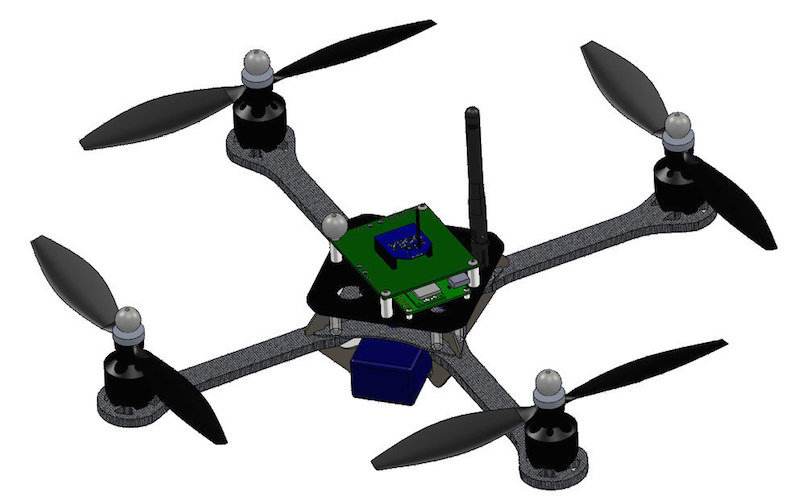
\includegraphics[width = 0.6 \textwidth]{img/quadrotor.jpg}
    \caption[Image of Quadrotor.]{Image of Quadrotor \cite{zainquad}.}
    \label{fig:quadrotor}
\end{figure}
Control systems are the foundation of devices which process inputs and produce a corresponding output. Open-loop control refers to control action, which is independent of the output, whereas closed-loop control refers to control action dependent on the output. Within the context of autonomous drone control, a closed-loop control system is essential in order to ensure the drone reacts to its external environment appropriately. The inputs of controllers for drones come from its sensors, such as gyroscopes, accelerometers, LIDAR, infrared and proximity sensors. The controllers for drones use the data from these sensors as inputs to the control system and output a corresponding signal to its motors, which in turn ensure the drone corrects its movement to changes in the external environment. The thrust, as well as rotation of the drone is responsible for its movement. The rotation is altered in three ways: pitch, roll and yaw. 

Pitch relates to the drone’s movement about its lateral axis, meaning a change in pitch will move the nose of the drone up or down. The pitch is controlled by changing the speed of the propellers at the front and back of the drone. Roll relates to the drone’s movement about its longitudinal axis, meaning a change in roll will tilt the drone. Roll is controlled by changing the speed of the propellers on the sides of the drone. Finally, yaw relates the drone’s movement around its vertical axis, which implies a change in yaw will turn the drone left or right. Yaw is controlled by changing the speeds of diagonal rotors.

There are many different types of control systems used in autonomous applications, with the state-of-the-art controller being a Proportional-Integral-Derivative (PID) controller. Research on new and improved control systems has been conducted over the past decade, with new controllers utilising Model Predictive Control (MPC) and learning-based control (such as neural networks) showing better performance in applications such as medical surgery, imagery and navigation \cite{zain11,zain9}. This improvement in performance is due to two reasons. Firstly, a PID controller requires mathematically modelling the drone’s dynamics and therefore can be computationally intensive for complex environments. Additionally, when mathematically modelling the drone’s dynamics, assumptions such as linearisation must be made which reduces the accuracy of the controller. In learning-based approaches where non-linearities can be accounted for, such as Artificial Neural Networks (ANN), the computational power required as well as accuracy can be improved. 

This project aims to implement a novel approach, using an Adaptive Neuro-Fuzzy Inference System (ANFIS) controller. This approach combines the benefits of using a neural network, with the benefits of fuzzy logic. Fuzzy logic allows for values in a universe to have an uncertain degree of membership and can therefore enable complex systems to be modelled in a less computationally demanding way. This approach has showed promising results within the context of other applications such as electrical conductivity prediction and control of medical devices \cite{boxi1,zain11}. Research within utilising ANFIS in the controllers of autonomous underwater vehicles has also provided a basis for further investigation in other applications. 

New commercially available software has applications and functions which allow ANFIS to be built in a more comprehensive and tailored way. In MathWorks release of MATLAB 2023a, they introduced a Fuzzy Logic Designer App which provides tools to design and tune complex fuzzy inference systems. The findings in literature, coupled with the advancements in software capabilities in this field, allow us to investigate using ANFIS in drone control.
 
\section{Research Problem}
The three issues associated with drones currently are: the cost, accuracy and reliability. Current commercial drones may solve one of these issues, or maybe two if considering accuracy and reliability. However, they have not yet effectively solved all three of these issues. Drone control is the key problem. PID controllers have drawbacks outlined in the project background which cause drone controllers to be computationally intensive. Therefore, this makes them larger and more expensive. Additionally, assumptions such as linearisation result in room for improvement in their control response. A learning based approach which is computationally efficient may allow all three parameters of success to be met. 
\section{Aims and Objectives}
The overall goal of this project is to design and implement an ANFIS (Adaptive Neuro-Fuzzy Inference System) to drone control and evaluate its effectiveness against PID control. The objectives and constraints are the following:

\begin{itemize}
  \item Build a simulation environment either from scratch or using existing simulators, in which parameters such as checkpoints and obstacles can be defined. The simulator should also allow for randomised simulation environments to increase the diversity of the datasets generated.
  \item Gather a dataset of greater than 500,000 datapoints (specified by our industry partners, MassiveAnalytic) with a wide range of simulation scenarios included, such that the drone training data encompasses simplified real world scenarios. 
  \item Perform data pre-processing methods using standard feature selection techniques. A training, validation and test dataset should be produced in order to adequately build and evaluate the ANFIS. 
  \item Build the ANFIS structure, using validation data to tune membership functions in order to minimise training and validation error. Justified ANFIS design decisions will be made to minimise testing error. 
  \item Implement the ANFIS into the simulator and test the ANFIS controller against the PID controller. The two performance metrics of error in position and computational power (number of Bytes of memory required) as well as computational time will be compared and evaluated.
  \end{itemize}

The main constraints relate to the limitations in software when designing the simulator and the ANFIS and computational power of the machine used to perform the data collection from the simulator. 
\begin{itemize}
  \item The more popular and commercially used simulation environments for drones such as Gazebo and ROS are difficult to integrate with the best software for building an ANFIS controller such as MATLAB and Python.
  \item Software that builds neuro-fuzzy inference systems is still being refined and improved. Hence, the resources available to design fuzzy inference systems and refine parameters such as the membership functions are limited. A key example of this is the inability to ``tune'' fuzzy inference systems with more than one output. For this project the Fuzzy Logic Designer Application released in MATLAB 2023a will be used however the 2024 version is likely to have improvements which we will be unable to incorporate.  
  \item As this is a fourth year project, there is a limited time frame (nine months) in which results have to be produced and refined therefore the depth of the analysis is limited. This constraint is particularly relevant to the optimal configuration and implementation of the controller as well as the size of the dataset used to train the ANFIS.
  \item Computational limitations when using personal laptops will be a constraint on the length and magnitude of the simulations and ANFIS built.  
  \end{itemize}
\section{Report Structure}
This report consists of six chapters where research, design and test the implementation of the ANFIS controller in a drone application is explored. 

\textbf{Chapter 1} - Presents the problems background as well as the aims and objectives of the project.

\textbf{Chapter 2} - A comprehensive literature review of the applications and success of neuro-fuzzy systems as well as the control methods currently used for drone dynamics. 

\textbf{Chapter 3} - Provides a detailed overview of the simulation environment created and reasoning for the assumptions and parameters chosen. 

\textbf{Chapter 4} - Explains the process and considerations when building and implementing the ANFIS system into the simulation environment. 

\textbf{Chapter 5} - Summarises and discusses the results of the various ANFIS configurations and the comparison between using the ANFIS controller versus the PID controller in the drone simulation. 

\textbf{Chapter 6} - Reflects on the findings and suggests possible future work.

Figure \ref{fig:generalFlow} shows the design methodology used in this project. 
\begin{figure}[H]
    \centering
    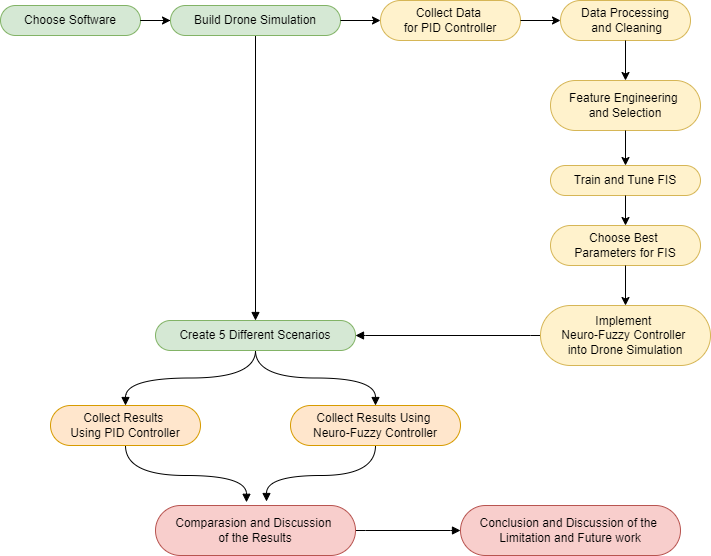
\includegraphics[width = 0.8 \textwidth]{img/generalflow.drawio.png}
    \caption{Flow Diagram of Methodology}
    \label{fig:generalFlow}
\end{figure}